\graphicspath{{images/act_1.2/}}
\subsection{Gravity and Coriolis compensation}
The objective of this activity is analyze effects of gravity and Coriolis terms on the relation between interaction torques ($\boldsymbol{\tau}_\mathbf{ext}$) and joint configuration ($\mathbf{q, \dot{q}, \ddot{q}}$). For this purpose, a simulation environment is developed that contains the UR5 robot and allows external torques to be applied. The simulation starts with initial joint configuration $\mathbf{q_0}=\begin{bmatrix} 0.0 & -1.0 & 1.0 & 0.5 & 0.0 & 0.5 \end{bmatrix}$ rad. Then, external torque $\tau_\mathrm{ext}= 20\sin{(2\pi t)}$ is applied to each joint. Finally, movements of ur5 robot is controlled with a proportional-derivative impedance control method with gravity compensation at joint level. Thus, control law can be computed as 
\begin{equation}
	\boldsymbol{\tau}
	= \mathbf{K_{des} e} + \mathbf{D_{des} \dot{e}} + \mathbf{b},
	\label{eq:articular_PDi_b}
\end{equation}
\noindent where $\mathbf{e}=\mathbf{q_{des} - q}$ is joint position error, $\mathbf{b}=\mathbf{C(q, \dot{q})} + \mathbf{g(q)}$ is nonlinear effects vector, and $\mathbf{D_{des}, K_{des}}$ are desired stiffness and damping matrix, respectively.

Figure \ref{fig:act1.2_tau_vs_q}-\ref{fig:act1.2_tau_vs_ddq} show relation between external force ($\tauext$) and joint configuration ($\jointconfiguration$) using control law \eqref{eq:articular_PDi_b} with $\mathbf{K_{des}}=500\eye$ $\mathrm{\frac{N.m}{rad}}$ and $\mathbf{D_{des}}=10\eye$ $\mathrm{\frac{N.m.s}{rad}}$. First, Figure \ref{fig:act1.2_tau_vs_q} shows relation between external torque ($\tauext$) and joint positions ($\mathbf{q}$). In this figure, impedance profiles are similar at end-tip unlike Figure \ref{fig:act1.1.3_tau_vs_q}. However, the profiles have different widths at middle. Second, Figure \ref{fig:act1.2_tau_vs_dq} shows relation between external torque ($\tauext$) and joint velocities ($\mathbf{\dot{q}}$). In this figure, impedance profiles are similar but not symmetrical. Finally, Figure \ref{fig:act1.2_tau_vs_ddq} shows relation between external torque ($\tauext$) and joint accelerations ($\mathbf{\ddot{q}}$). In this figure, impedance profiles have different widths at middle and shapes at end-tip. The differences in impedance profiles ($\tauext$ vs $\jointconfiguration$) are generated because the ur5 robot generates different inertia effects on each joint. Finally, impedance profiles can be improved by compensating for inertial effects at control law.


\begin{figure}
\centering
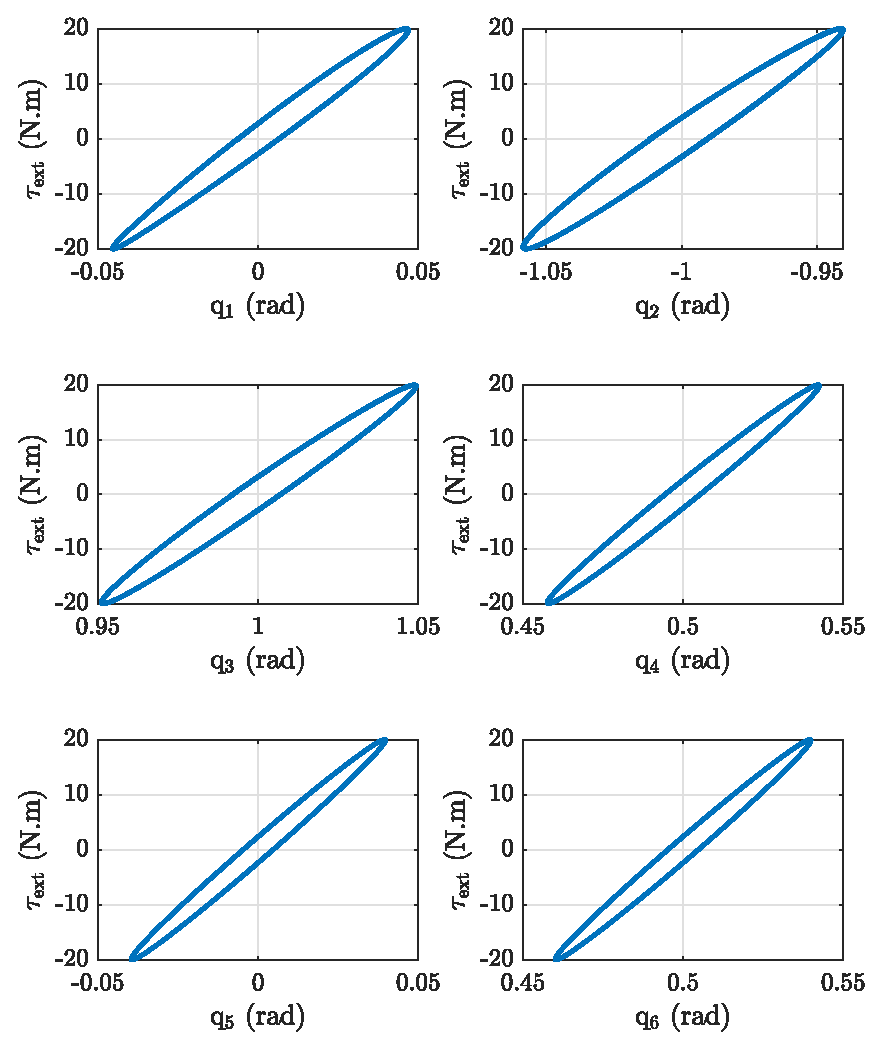
\includegraphics{external_torque_vs_joint_position.eps}
\caption{Dynamic relation between external torque ($\tauext$) and joint positions ($\mathbf{q}$) using proportional-derivative impedance control with gravity compensation \eqref{eq:articular_PDi_b} with $\mathbf{K_{des}}=500\eye$ $\mathrm{\frac{N.m}{rad}}$ $\mathbf{D_{des}}=10\eye$ and $\mathrm{\frac{N.m.s}{rad}}$.}
\label{fig:act1.2_tau_vs_q}
\end{figure}

\begin{figure}
\centering
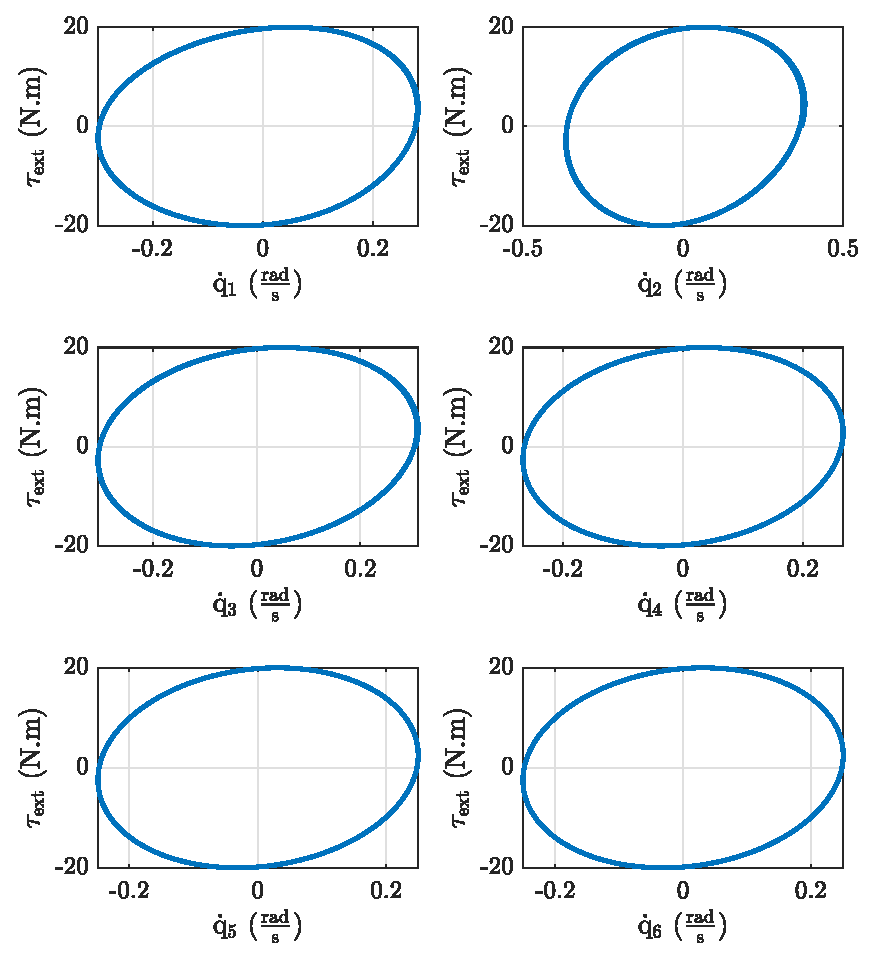
\includegraphics{external_torque_vs_joint_velocity.eps}
\caption{Dynamic relation between external torque ($\tauext$) and joint velocities ($\mathbf{\dot{q}}$) using proportional-derivative impedance control with gravity compensation \eqref{eq:articular_PDi_b} with $\mathbf{K_{des}}=500\eye$ $\mathrm{\frac{N.m}{rad}}$ $\mathbf{D_{des}}=10\eye$ and $\mathrm{\frac{N.m.s}{rad}}$.}
\label{fig:act1.2_tau_vs_dq}
\end{figure}

\begin{figure}
\centering
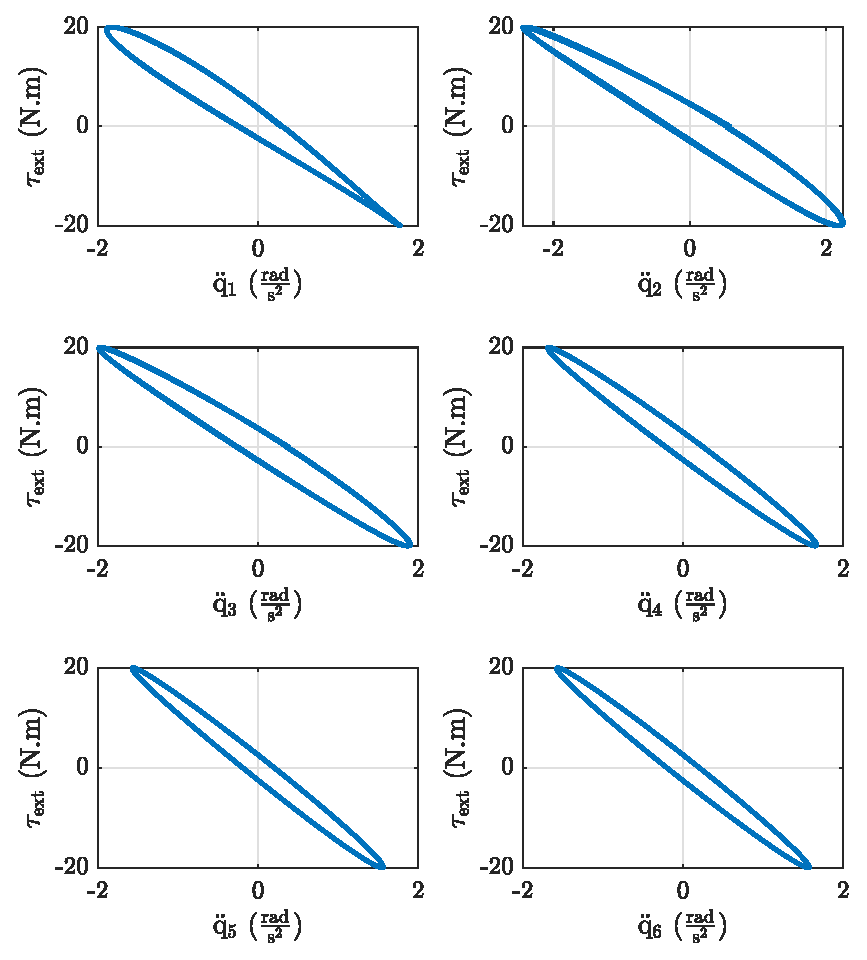
\includegraphics{external_torque_vs_joint_acceleration.eps}
\caption{Dynamic relation between external torque ($\tauext$) and joint accelerations ($\mathbf{\ddot{q}}$) using proportional-derivative impedance control with gravity compensation \eqref{eq:articular_PDi_b} with $\mathbf{K_{des}}=500\eye$ $\mathrm{\frac{N.m}{rad}}$ $\mathbf{D_{des}}=10\eye$ and $\mathrm{\frac{N.m.s}{rad}}$.}
\label{fig:act1.2_tau_vs_ddq}
\end{figure}
